\documentclass[border=2pt]{standalone}
\usepackage{amsmath}
\usepackage{tikz}
\usetikzlibrary{intersections}
\usetikzlibrary{arrows}
\usetikzlibrary{quotes,angles}
\usepackage{amsmath}
\usepackage{xcolor}

\begin{document}

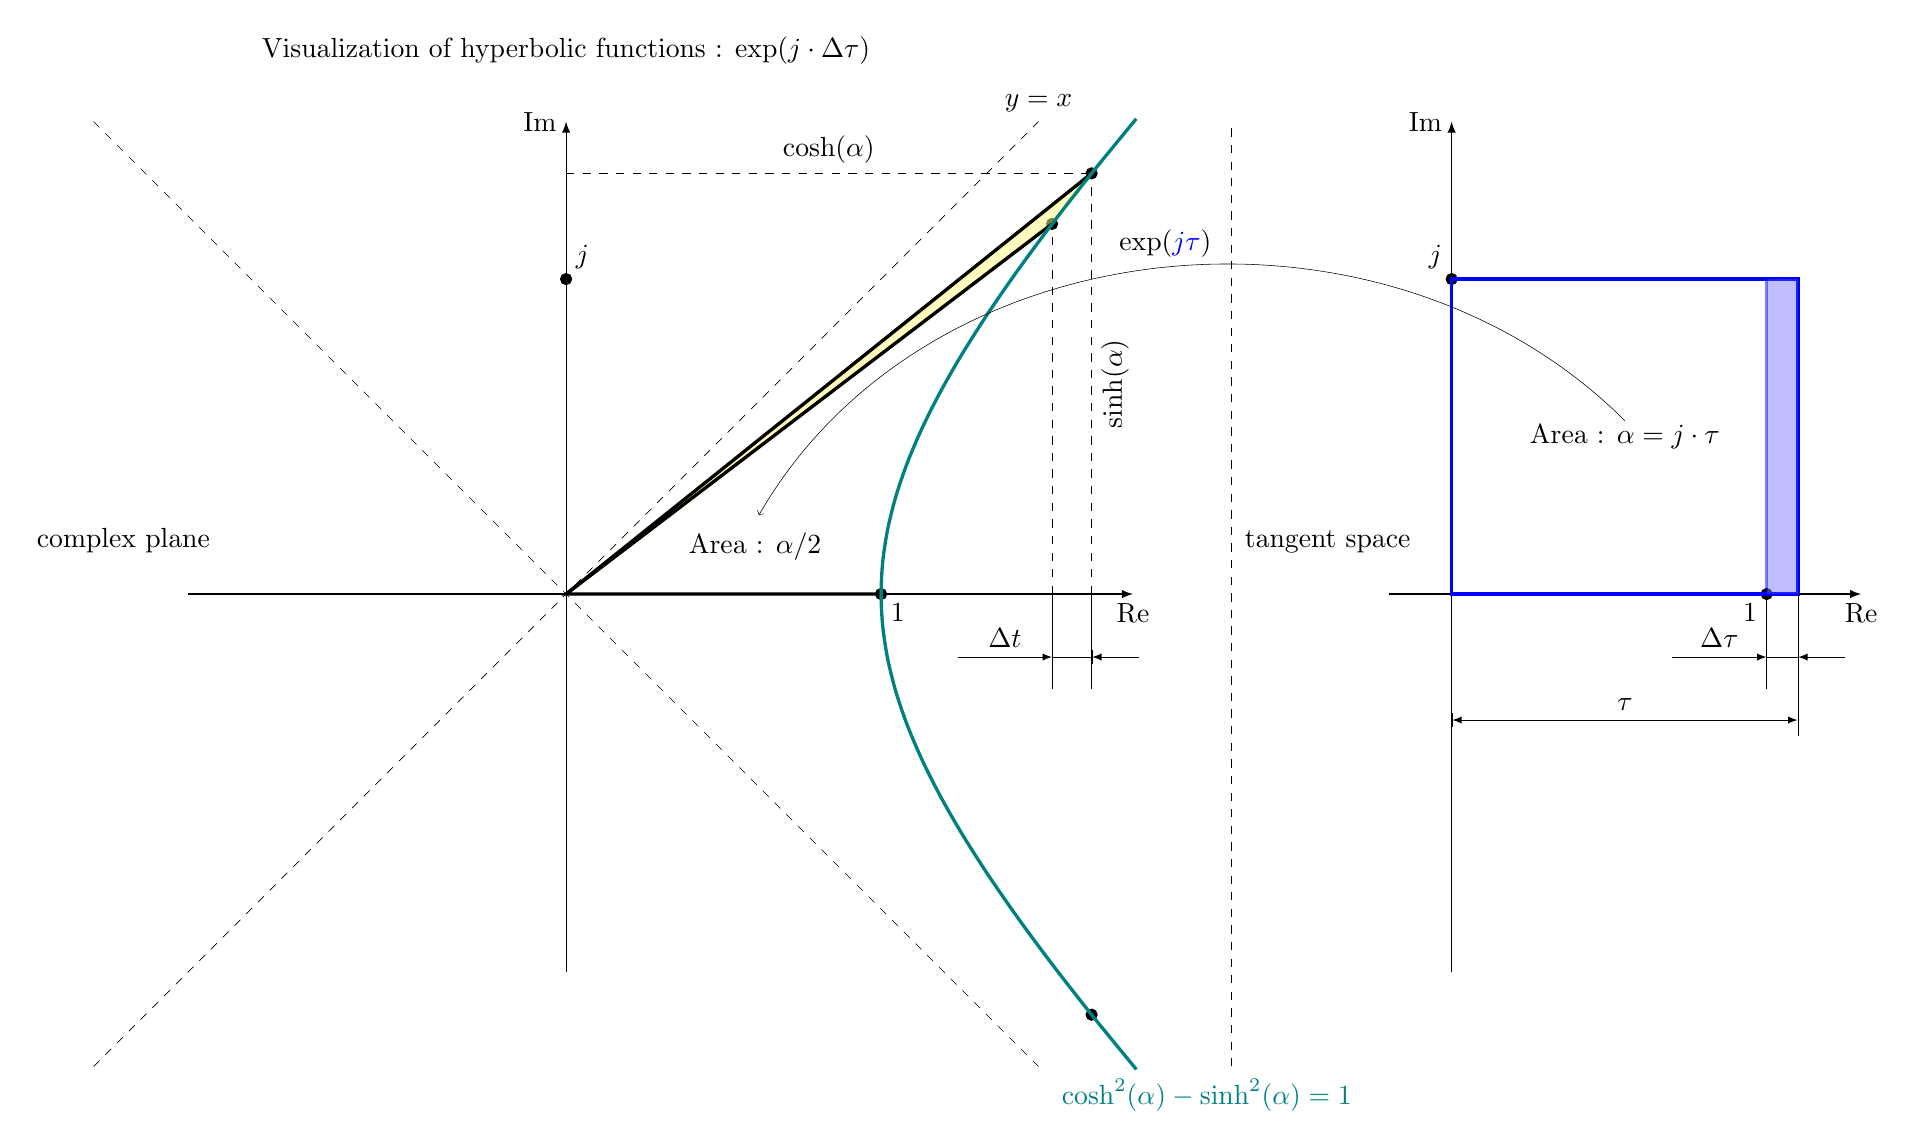
\begin{tikzpicture}[scale=4]

% Draw x and y axis lines
\draw [->,>=latex] (-1.2,0) -- (1.80,0) node [below] {$\mathrm{Re}$};
\draw [->,>=latex] (0,-1.2) -- (0,1.50) node [left ] {$\mathrm{Im}$};
\node[above left] at (-1.1, 0.1) {complex plane};
\filldraw[black] (1,0) circle (0.5pt) node[below right] {$1$} ;
\filldraw[black] (0,1) circle (0.5pt) node[above right] {$j$} ;
\node[above] at (0.0,1.65) {Visualization of hyperbolic functions : $\exp(j \cdot \Delta\tau)$};

% Draw a circle at the origin of radius 1
%\draw (0,0) circle (1);

\draw [very thin, dashed] (-1.5,-1.5) -- ( 1.5, 1.5) node[above] {$y=x$} ;
\draw [very thin, dashed] (-1.5, 1.5) -- ( 1.5,-1.5) ;

\pgfmathsetmacro{\angle}{1.1}
\pgfmathsetmacro{\length}{\angle}
\pgfmathsetmacro{\dangle}{0.1}
\pgfmathsetmacro{\dlength}{\dangle}

\filldraw[black] ({ cosh(\angle)}, { sinh(\angle)}) circle (0.5pt) ;
\filldraw[black] ({ cosh(\angle)}, {-sinh(\angle)}) circle (0.5pt) ;
\filldraw[black] ({ cosh(\angle-\dangle)}, { sinh(\angle-\dangle)}) circle (0.5pt) ;

\draw [very thin, dashed] ( 0.0, { sinh(\angle)}) -- node[above] {$\cosh(\alpha)$} ({ cosh(\angle)}, { sinh(\angle)}) ;
\draw [very thin, dashed] ( { cosh(\angle)}, 0.0) -- node[below, rotate=90] {$\sinh(\alpha)$} ({ cosh(\angle)}, { sinh(\angle)}) ;
\draw [very thin, dashed] ( { cosh(\angle-\dangle)}, 0.0) -- ({ cosh(\angle-\dangle)}, { sinh(\angle-\dangle)}) ;

\filldraw[very thick, draw=yellow,fill=yellow!50,opacity=0.5]
[smooth,variable=\x] plot[domain=\angle-\dangle:\angle] ({ cosh(\x)}, {sinh(\x)})
 -- ({ cosh(\angle)}, { sinh(\angle)}) -- (0,0) -- ({ cosh(\angle-\dangle)}, { sinh(\angle-\dangle)})
;
\draw[very thick, black] ({ cosh(\angle)}, { sinh(\angle)}) -- (0,0) -- (1,0) ;
\draw[very thick, black] ({ cosh(\angle-\dangle)}, { sinh(\angle-\dangle)}) -- (0,0) ;

% 画双曲线
\draw[very thick,smooth,variable=\x, color=teal] plot[domain=-\angle-\dangle:\angle+\dangle] ({ cosh(\x)}, {sinh(\x)}) ;
\node[below right, teal] at ({ cosh(\angle-0.1)}, {-sinh(\angle+0.1)}) {$\cosh^2(\alpha) - \sinh^2(\alpha) = 1$} ;
%\draw[very thick,smooth,variable=\x, color=blue] plot[domain=-1.2:1.2] ({-cosh(\x)}, {sinh(\x)}) ;

% Draw a string at center.
\node at (0.6, 0.15) {Area : $\alpha/2$};

\draw [very thin] ( { cosh(\angle)}, 0.0) -- ({ cosh(\angle)}, -0.30) ;
\draw [very thin] ( { cosh(\angle-\dangle)}, 0.0) -- ({ cosh(\angle-\dangle)}, -0.30) ;
\draw [very thin, ->,>=latex] ({ cosh(\angle-\dangle)-0.3}, -0.2) -- node[above] {$\Delta t$} ({ cosh(\angle-\dangle)}, -0.2);
\draw [very thin] ({ cosh(\angle-\dangle)}, -0.2) -- ({ cosh(\angle)}, -0.2) ;
\draw [very thin, |<-,>=latex] ({ cosh(\angle)}, -0.2) -- ({ cosh(\angle)+0.15}, -0.2) ;


\begin{scope}[xshift=80]

\draw [very thin, dashed] (-0.7,-1.5) -- (-0.7, 1.50) ;
\draw [->,>=latex] (-0.2,0) -- (1.30,0) node [below] {$\mathrm{Re}$};
\draw [->,>=latex] (0,-1.2) -- (0,1.50) node [left ] {$\mathrm{Im}$};
\node[above left] at (-0.1, 0.1) {tangent space};
\filldraw[black] (1,0) circle (0.5pt) node[below left] {$1$} ;
\filldraw[black] (0,1) circle (0.5pt) node[above left] {$j$} ;

\draw[very thick,draw=blue] (0,0) rectangle (\length, 1);
\filldraw[very thick,draw=blue,fill=blue!50,opacity=0.5] (\length,0) rectangle (\length-\dlength, 1);
%\draw[very thick,draw=red] (\length,0) rectangle (\length-\dlength, 1);
\draw [very thin] (\length, 0.0) -- (\length, -0.45);
\draw [very thin, |<->|,>=latex] ( 0.0, -0.4) -- node[above] {$\tau$} (\length, -0.4);
\draw [very thin, ->,>=latex] (\length-\dlength-0.3, -0.2) -- node[above] {$\Delta\tau$} (\length-\dlength, -0.2);
\draw [very thin] (\length-\dlength, -0.2) -- (\length, -0.2) ;
\draw [very thin, <-,>=latex] (\length, -0.2) -- (\length+0.15, -0.2) ;
\draw [very thin] (\length-\dlength, -0.0) -- (\length-\dlength, -0.30) ;

\node at (\length/2, 1/2) {Area : $\alpha = j \cdot \tau$};

\draw [very thin, ->] (\length/2, 1/2+0.05) to [out=135,in=60] node[above ] {$\exp(\color{blue}j\tau\color{black})$}  (-2.20, 0.25);

\end{scope}


\end{tikzpicture}

\end{document}
